%Modified from a template provided by Jennifer Pan, August 2011

\documentclass[10pt,letter]{article}
	% basic article document class
	% use percent signs to make comments to yourself -- they will not show up.
\usepackage{pdfsync}
\usepackage{amsmath}
\usepackage{amssymb}
\usepackage{amsthm}
\usepackage{ mathrsfs }
	% packages that allow mathematical formatting


\usepackage{graphicx}
	% package that allows you to include graphics
\graphicspath{ {./images/} }

\usepackage{setspace}
	% package that allows you to change spacing

\onehalfspacing
	% text become 1.5 spaced

\usepackage{fullpage}
% package that specifies normal margins

\usepackage[parfill]{parskip}

\usepackage{cancel}

\newtheorem*{thm}{Theorem}
\newtheorem{nthm}{Theorem}

\begin{document}
	% line of code telling latex that your document is beginning

\title{Problem Set 6: CS103}

\author{Katherine Cheng, Richard Davis, Marty Keil}

% \date{Friday April 10, 2015}
	% Note: when you omit this command, the current date is automatically included
 
\maketitle
	% tells latex to follow your header (e.g., title, author) commands.

\section*{Problem 1: The Myhill-Nerode Theorem}
\paragraph{i}
\begin{thm} L is a regular language, where $\Sigma = \{a,b\}$ and $L=\{w \in \Sigma^* |\ |w| \text{ is even}\}$\end{thm}
\begin{proof}

Let $\Sigma = \{a,b\}$ and let $L=\{w \in \Sigma^* |\ |w| \text{ is even}\}$. We can design DFA for this language:

\begin{figure}[h]
    \centering
    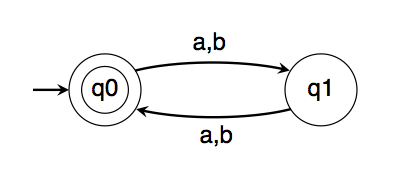
\includegraphics[width=0.4\linewidth]{hw6_1i.png}
    \caption{DFA for the language $L=\{w \in \Sigma^* |\ |w| \text{ is even}\}$ where $\Sigma = \{a,b\}$}
    \label{fig:q1i}
\end{figure}

As defined in lecture, we know that a language $L$ is a regular language if there exists a DFA $D$ such that $\mathscr{L}(D) =L$. Thus, L must be a regular language.
\end{proof}

\paragraph{ii}
\begin{thm} There is an infinite set $S \subseteq \Sigma^*$ where there are infinitely many pairs of distinct strings $x, y \in S$ such that $x\ \cancel{\equiv}_L\ y$ \end{thm}

\begin{proof}
Let $S= \{a^n\ |\ n \in \mathbb{N}\}$. This set is infinite because it contains one string for each natural number. Since $a^n$ is the string $a$ concatenated to itself $n$ times, we know the length of $a^n$ is $n$. Now, consider any pair of strings $a^n, a^{n+1} \in S$. The lengths of these strings are $n$ and $n+1$ respectively. By the definition of even and odd numbers, if $n$ is even, $n+1$ must be odd. If $n$ is odd, $n+1$ must be even. In either case, one string in the pair must be even-length and in the language $L$, and the other odd-length and not in the language $L$, meaning that $a^n\ \cancel{\equiv}_L\ a^{n+1}$. There are infinite such pairs, thus, S has infinitely many pairs of distinct strings.
\end{proof}

\paragraph{iii}
\begin{thm} There is no infinite set $S \subseteq \Sigma^*$ where all pairs of distinct strings $x,y\in S$ satisfy $x\ \cancel{\equiv}_L\ y$ \end{thm}

\begin{proof}
By contradiction. Suppose there is an infinite set $S \subseteq \Sigma^*$ where all pairs of distinct strings $x,y \in S$ satisfy $x\ \cancel{\equiv}_L\ y$. We know that every string must be of even or odd length. If we take any three distinct strings from the infinite set S, by the pigeonhole principle, we know that two of these strings are of odd length, or two of these strings are of even length. Thus, we have found a pair of distinct strings where $x \equiv_L y$. We have reached a contradiction, so our original assumption must be false. Thus, there is no infinite set $S \subseteq \Sigma^*$ where all pairs of distinct strings $x,y\in S$ satisfy $x\ \cancel{\equiv}_L\ y$
\end{proof}

\section*{Problem 2: Balanced Parentheses}
\paragraph{i}
\thm The Language L = ( $w \in \Sigma*$ $\mid$ w is a string of balanced parentheses ) is not regular. 

\begin{proof}
Let $S = \{ (^n\ |\ n \in N$\}. This set is infinite because it contains one string of parentheses with length for each natural number. Now consider any strings $(^x$, $(^y$ $\in$ S where $(^x$ $\neq$ $(^y.$  One can add w, a  string with closing parentheses, ),  equal to the number of string x open parentheses. This can also be written as $)^x$. If this is the case, then  $(^xw \in L$ and $(^yw \notin L.$  $(^yw$ is not closed because there are an unequal number of open and closed parentheses. Consequently, X is distinguishable from y. Therefore, by the Myhill-Nerode theorem, L is not regular. \\ \\
\end{proof}

\paragraph{ii} DFA 

\begin{figure}[h]
    \centering
    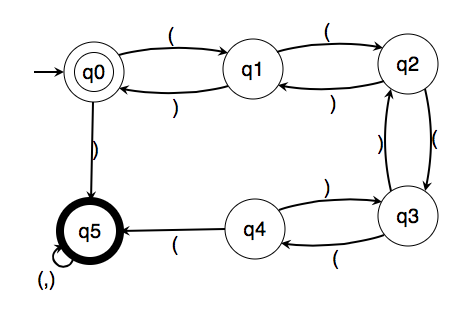
\includegraphics[width=0.4\linewidth]{p2ii}
    \caption{DFA for the language L = ( w $\in$ $\Sigma*$ $\mid$ w is a string of balanced parentheses and nesting length of at most 4)}
    \label{fig:q1i}
\end{figure}

\paragraph{iii} Context Free Grammar \\
\begin{figure}[h]
    \centering
    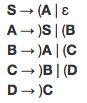
\includegraphics[width=0.15\linewidth]{p2iii}
    \caption{Context Free Grammar for L2}
    \label{fig:q1i}
\end{figure}

\section*{Problem 3: Subsets of Regular Languages}
Let $\Sigma = \{a, b\}$ and let $L = \{ w \in \Sigma^* \ | \ w \text{ has the same number of a's and b's} \}$. 

\paragraph{i.} 
\begin{thm} $L$ is not a regular language. \end{thm}

\begin{proof}
Let $S \subseteq \Sigma^*$ and define $S = \{a^n \ | \ n \in \mathbb{N} \}$. This set is infinite because it contains one string for every natural number. Now, consider any strings $a^m, a^n \in S$ where $a^m \not = a^n$. Then $a^n b^n \in L$ and $a^m b^n \not \in L$. Consequently, $a^n \not \equiv_L a^m$. Therefore, by the Myhill-Nerode theorem, $L$ is not regular.

Note that the structure of this proof was taken from slide 41 of Small16.pdf.
\end{proof}

\paragraph{ii.}
The language $L' = \{ (ab)^n \ | \ n \in \mathbb{N} \}$ is a subset of $L$. This language is infinite because it contains one string for every natural number. However, this language is regular because it can be defined using the regular expression \texttt{(ab)*}. 

\paragraph{iii.}
\begin{thm} There is no language $L' \subseteq  \{a^nb^n \ | \ n \in \mathbb{N} \}$ that contains infinitely many strings and is a regular language. \end{thm}
\begin{proof}
In the class slides we proved that the language $L = \{a^nb^n \ | \ n \in \mathbb{N} \}$ is irregular by showing that the language is infinite and that all of the strings in the language are pairwise distinguishable. Because all of the strings in this language are pairwise distinguishable, we can choose any subset of $L$ and we know that all of the strings in that subset will be pairwise distinguishable. We choose an arbitrary infinite subset of $L$ called $S'$. Since $S'$ is both infinite and all the strings in it are pairwise distinguishable, by the Myhill-Nerode theorem we know it is an irregular language. If any arbitrary infinite subset of $L$ is irregular, then we know that there is no language $L' \subseteq  = \{a^nb^n \ | \ n \in \mathbb{N} \}$ that contains infinitely many strings and is a regular language.
\end{proof}

\section*{Problem 4: State Lower Bounds}
\paragraph{i}
\begin{thm}Any DFA for L, where L is a language over $\Sigma$ and there's a finite set S such that any two distinct strings $x,y\in S$ are distinguishable relative to L, must have at least $|S|$ states. \end{thm}

\begin{proof} Let the number of strings in set S, $|S| = k$. Since all pairs of distinct strings x and y are pairwise distinguishable relative to L, by the definition of distinguishability discussed in lecture, any DFA for L must end in different states when run on inputs x and y. If every input string leads the DFA for L to end in a different state from every other string, each input string must lead the DFA to a unique state. Thus, if there are k strings in set S, there are at least k states in the DFA for L. Substituting $|S|$ back in for k, this means that any DFA for L must have at least $|S|$ states.
\end{proof}

\paragraph{ii}
\begin{thm} The following DFA is the smallest possible DFA for L, where L is a language over $\Sigma = \{a,b\}$ and $L=\{w \in \Sigma^*\ |\ |w| \equiv_4 2\}$.\end{thm}

\begin{figure}[h]
    \centering
    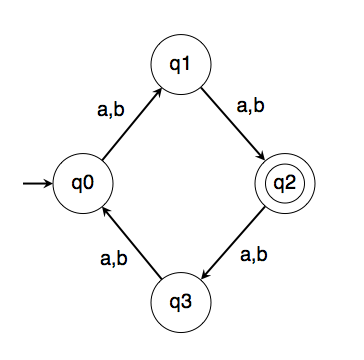
\includegraphics[width=0.4\linewidth]{hw6_4ii.png}
    \caption{DFA for the language $L=\{w \in \Sigma^*\ |\ |w| \equiv_4 2\}$ where $\Sigma = \{a,b\}$}
    \label{fig:q4ii}
\end{figure}

\begin{proof} Assume L is a language over $\Sigma = \{a,b\}$ and $L=\{w \in \Sigma^*\ |\ |w| \equiv_4 2\}$. We will show that the DFA modeled here is the smallest possible DFA for L, the measure of ``smallest" being the number of states in the DFA (which, in this DFA, is 4 states). 

Take the finite set, $S = \{a^1, a^2, a^3, a^4\}$. We can take any pair of strings $a^n, a^m \in S$ and add a string w to each, where $w = a^{6-n}$. Adding w to these strings will lead exactly one string, $a^n + w = a^n+a^{6-n} = a^6$, to be in L ($a^6 \equiv_4 2$), and the other not to be in L. Thus, as defined in lecture, the strings $a^n, a^m \in S$ are distinguishable relative to L. Since this is true of any pair of strings in S, the strings in this finite set are all pairwise distinguishable relative to L.

By our proof in Part i of this problem, since we have shown there is a finite set S such that all strings in the set are pairwise distinguishable relative to L, there must be at least $|S|$ states in the DFA for L. The cardinality of our set S is 4, so there must be at least 4 states in the DFA for L. Therefore, our DFA depicted above must be the smallest possible DFA for L. 
\end{proof}

\section*{Problem 5: Closure Properties Revisited}
\paragraph{i.}
\begin{thm} The nonregular languages are closed under complementation. \end{thm}
\begin{proof}
By contradiction. Assume for the sake of contradiction that there exists some nonregular language $L$ whose complement is a regular language $L'$. From the class slides, we know that the complement of any regular language is a regular language. So, because $L'$ is a regular language, its complement $L$ must also be a regular language. However we defined $L$ as nonregular. This is a contradiction, which means our assumption that there exists some nonregular language $L$ whose complement is a regular language must be false. So the nonregular languages are closed under complementation.
\end{proof}

\paragraph{ii.}
\begin{thm} The nonregular languages are not closed under union. \end{thm}
\begin{proof} We will show that there are two nonregular languages whose union is regular. Let $\Sigma = \{a, b\}$ and $L = \{a^nb^n \ | \ n \in \mathbb{N} \}$. We know that $L$ is nonregular. Let $L'$ be the complement of $L$. From the previous proof we know that $L'$ must be nonregular as well. The union of these two languages is the language that accepts any string in $\Sigma^*$: if the string is not accepted by $L$, then by definition of complementation it must be accepted by $L'$. This language can be represented by a DFA with a single accepting state that is also the start state with self-transitions on both $a$ and $b$. Because this language can be represented by a DFA, this means it is regular. Thus, the nonregular languages are not closed under union.
\end{proof}

\paragraph{iii.}
\begin{thm} The regular languages are not closed under infinite union. \end{thm}
\begin{proof}
We will prove that it is possible to construct a nonregular language from an infinite union of regular languages, proving that the regular languages are not closed under infinite union. We can define an infinite set of regular languages $L^n = \{a^n b^n\}$ for every natural number. Because each of these languages only accepts a single string, we know that each can be defined by a regular expression, making each a regular language. However, the union of these languages is $L = \{ a^n b^n \ | \ n \in \mathbb{N} \}$. We know from an earlier proof that this language is nonregular. This proves that the regular languages are not closed under infinite union.
\end{proof}

\section*{Problem 6: Designing CFGs}
\paragraph{i} CFG: \\
Start Symbol: S \\
S $\rightarrow$ $\mathcal{E}$ $\mid$ XaaX \\
X $\rightarrow$ $\mathcal{E}$ $\mid$ bX $\mid$ cX $\mid$ aX \\

Derivations: \\
\textbf{\underline{aa}} \\
S\\
$\rightarrow$ XaaX \\
$\rightarrow$ aaX \\
$\rightarrow$ aa

\textbf{\underline{baac}} \\
S\\
$\rightarrow$ XaaX \\
$\rightarrow$ bXaaX \\
$\rightarrow$ baaX \\
$\rightarrow$ baacX \\
$\rightarrow$ baac 

\textbf{\underline{ccaabb}} \\ 
S\\
$\rightarrow$ XaaX \\
$\rightarrow$ cXaaX \\
$\rightarrow$ ccXaaX \\
$\rightarrow$ ccXaaX \\
$\rightarrow$ ccaaX \\
$\rightarrow$ ccaabX \\
$\rightarrow$ ccaabbX \\
$\rightarrow$ ccaabb 


\paragraph{ii} CFG: \\
Start Symbol: S\\
S $\rightarrow$ aSa $\mid$ bSb $\mid$ aSb $\mid$ bSa $\mid$ T \\
T $\rightarrow$ aUb $\mid$ bUa \\
U $\rightarrow$ aUa $\mid$ bUb $\mid$ aUb $\mid$ bUa $\mid$ a $\mid$ b $\mid$ $\mathcal{E}$ \\

Derivations: \\
\textbf{\underline{aab}} \\
S\\
$\rightarrow$ T \\
$\rightarrow$ aUb \\
$\rightarrow$ aab 

\textbf{\underline{abbaba}} \\
S\\
$\rightarrow$ aSa \\
$\rightarrow$ abSba \\
$\rightarrow$ abTba \\
$\rightarrow$ abbUaba \\
$\rightarrow$ abbaba \\


\paragraph{iii} CFG: \\
Start Symbol: S\\
S $\rightarrow$ 1S1 $\mid$ T \\
T $\rightarrow$ +U \\
U $\rightarrow$ 1U1 $\mid$ $\stackrel{?}{=}$

Derivations:\\
\textbf{\underline{111+1 $\stackrel{?}{=}$1111}} \\
S\\
$\rightarrow$1S1 \\
$\rightarrow$11S11 \\
$\rightarrow$111T111 \\
$\rightarrow$111+U111 \\
$\rightarrow$111+1U1111 \\
$\rightarrow$111+1 $\stackrel{?}{=}$1111



\textbf{\underline{+1$\stackrel{?}{=}$1}} \\
S\\
$\rightarrow$ T\\
$\rightarrow$ +U\\
$\rightarrow$ +1U1\\
$\rightarrow$ +1$\stackrel{?}{=}$1

\paragraph{iv} CFG: \\
Start symbol: S \\
S $\rightarrow$ aSXXX $\mid$ bXXX $\mid$ SXXXX \\
X $\rightarrow$ a $\mid$ b

Derivations: \\
\textbf{\underline{baaa}} \\
S\\
$\rightarrow$ bXXX \\
$\rightarrow$ baXX \\
$\rightarrow$ baaX \\
$\rightarrow$ baaa

\textbf{\underline{abaaaaaa}} \\
S\\
$\rightarrow$ aSXXX \\
$\rightarrow$ abXXXXXX \\
$\rightarrow$ abaXXXXX \\
$\rightarrow$ abaaXXXX \\
$\rightarrow$ abaaaXXX \\
$\rightarrow$ abaaaaXX \\
$\rightarrow$ abaaaaaX \\
$\rightarrow$ abaaaaaa 

\textbf{\underline{baaaaaaa}} \\
S \\
$\rightarrow$ SXXXX \\
$\rightarrow$ bXXXXXXX \\
$\rightarrow$ baXXXXXX \\
$\rightarrow$ baaXXXXX \\
$\rightarrow$ baaaXXXX \\
$\rightarrow$ baaaaXXX \\
$\rightarrow$ baaaaaXX \\
$\rightarrow$ baaaaaaX \\
$\rightarrow$ baaaaaaa 

\paragraph{v} CFG: \\
Start Symbol: S \\
S $\rightarrow$ ySd $\mid$ dSyySd $\mid$ ySddSy $\mid$ dSy $\mid$ $\mathcal{E}$

Derivations: \\
\textbf{\underline{yyyddd}} \\
S \\
$\rightarrow$ ySd \\
$\rightarrow$ yySdd \\
$\rightarrow$ yyySddd \\
$\rightarrow$ yyyddd

\textbf{\underline{ydyd}} \\
S \\
$\rightarrow$ ySd \\
$\rightarrow$ ydSyd \\
$\rightarrow$ ydyd

\textbf{\underline{yyddddyy}} \\
S \\
$\rightarrow$ ySddSy \\
$\rightarrow$ yySdddSy \\
$\rightarrow$ yydddSy \\
$\rightarrow$ yyddddSyy \\
$\rightarrow$ yyddddyy
\end{document}
%%% Local Variables:
%%% mode: latex
%%% TeX-master: t
%%% End:
